

\documentclass[colorlinks=true,pdfstartview=FitV,linkcolor=blue,
            citecolor=red,urlcolor=magenta]{ligodoc}

\usepackage{graphicx}
\usepackage{amssymb}
\usepackage{amsmath}
\usepackage{longtable}
\usepackage{rotating}
\usepackage[usenames,dvipsnames]{color}
\usepackage{fancyhdr}
\usepackage{subfigure}
\usepackage{hyperref}
\ligodccnumber{T}{11}{XXXXX}{}{vX}% \ligodistribution{AIC, ISC}


\title{Online Detector Characterization using Neural Networks}

\author{Roxana Popescu}


\begin{document}

\section{Introduction} 
\par The data obained from LIGO has noise that comes from many sources. In order to be be able to better distinguish a signal from the noise is it is important to characterize the type of noise observed. Neural networks can be used to characterize the noise.

\par Neural networks can be used to find relationships between the inputed data using hidden layers of connections within the data. A diagram of a neural network is shown in Figure \ref{fig:image1}.

\par  Recurrent neural networks are neural networks that use  loops within them so that previous information can be retained. Long Short Term Memory (LTSM) networks are a type of recurrent neural network that can remeber information for longer than a typical recurrent neural network. A diagram of a LTSM network is shown in Figure \ref{fig:image2}. 

\begin{figure}[htbp]
\begin{center}
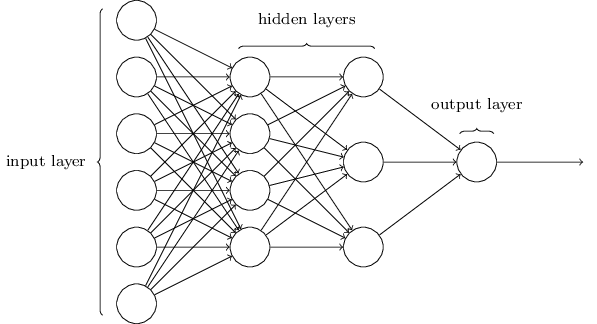
\includegraphics[width=5in]{neuralnetwork.png}
\caption{Diagram of Neural Network (from \url{http://neuralnetworksanddeeplearning.com/chap1.html})}
\label{fig:image1}
\end{center}
\end{figure}    

\begin{figure}[htbp]
\begin{center}
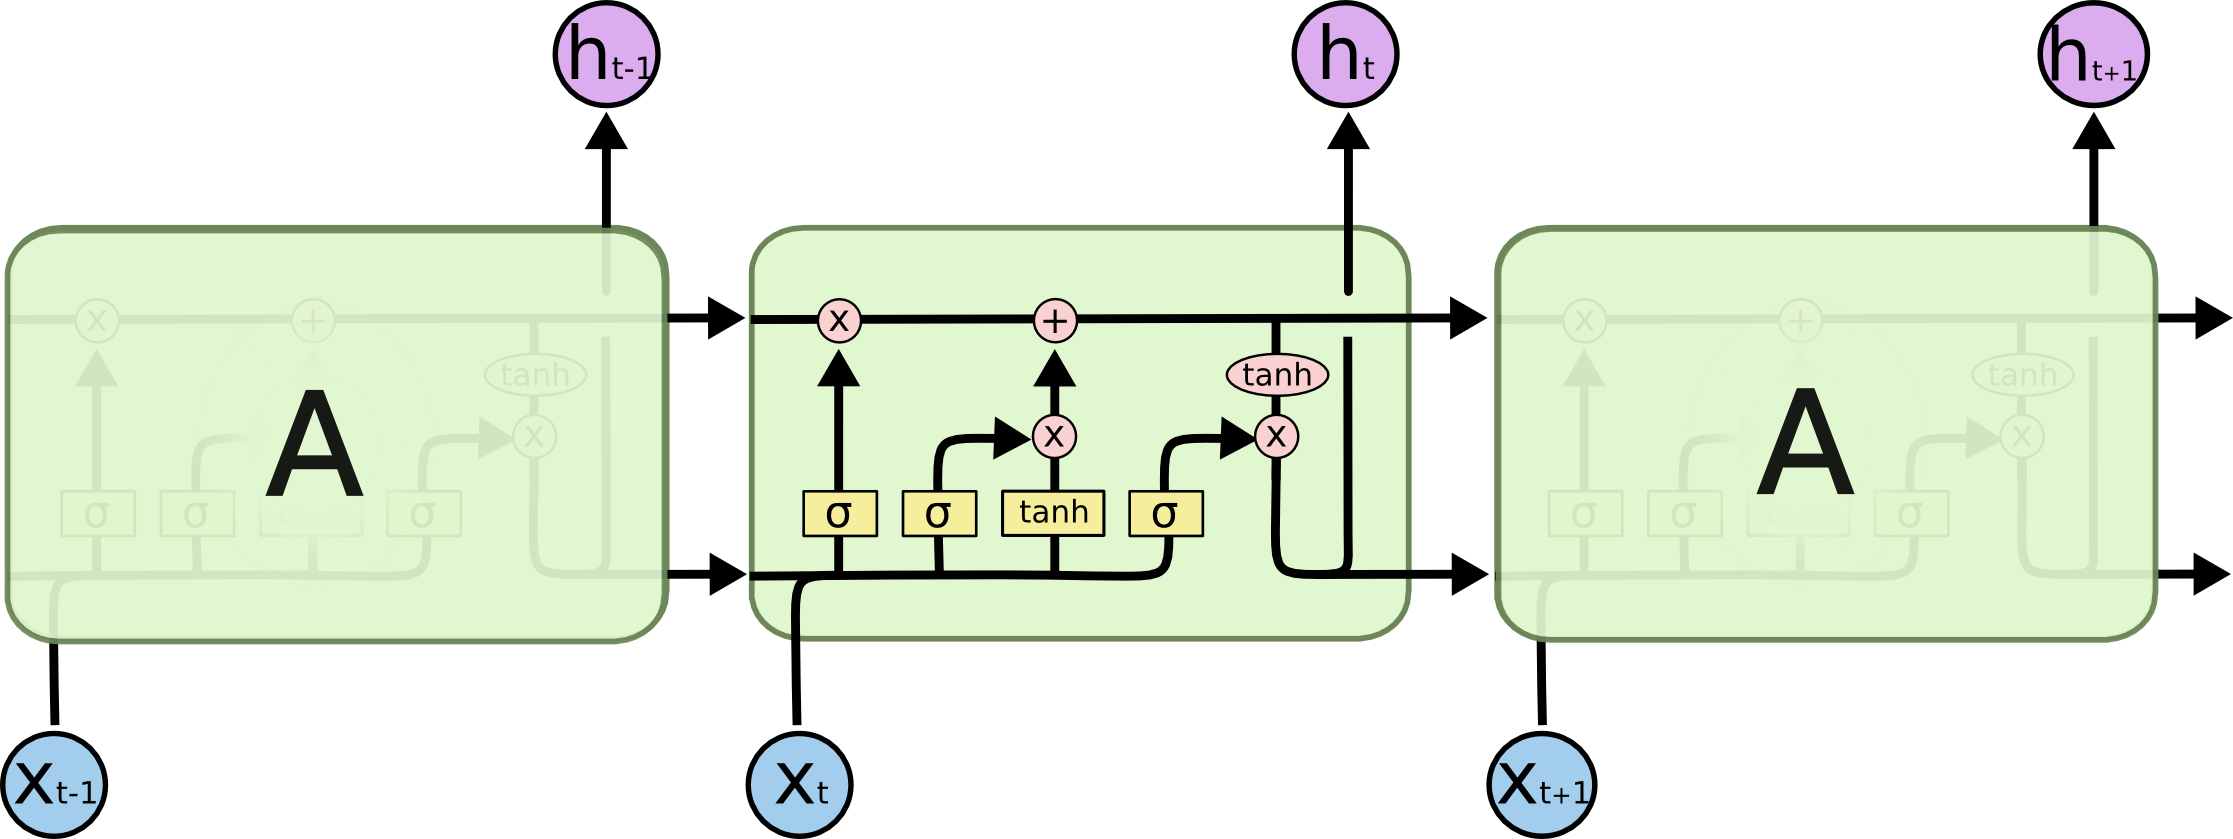
\includegraphics[width=5in]{ltsm.png}
\caption{Diagram of LTSM (from \url{http://colah.github.io/posts/2015-08-Understanding-LSTMs)}}
\label{fig:image2}
\end{center}
\end{figure}   

\section{Classification vs. Clustering}

In order to sort data two types of approaches are used: classification and clustering. Classification algorithms search the data and sort the data into already defined categories. Clustering algorithms look for relationships within the data to create categories into which the data is sorted. Classification algorithms are part of supervised learning since the computer determines the structure of the data from data that is already provided. Clustering algorithms are part of unsupervised learning since the computer determines the structure of the data without any previous information.  Clustering algorithms can be used to characterize the noise by identifying common characteristics within the noise depending on its sources. Clustering algortithms can further help with classification. A summary of the differences between classification and clusteirng is shown in the table below.

\begin{center}
 \begin{tabular}{|c | c|} 
 \hline
 Classification & Clustering\\ [0.5ex] 
 \hline\hline
 Supervised Learning & Unsupervised Learning\\ 
 \hline
 Classes are known & Classes are unknown\\
 \hline
 Used to classify data & Used to find relationships within data\\
 \hline
\end{tabular}
\end{center}

\par An example of  a clustering visualization code can be found at \url{https://www.mathworks.com/help/stats/visualize-high-dimensional-data-using-t-sne.html}.

\section{Objectives}  
The interferometer's gravitational wave signal output is a time series. We will see whether to analyze the raw time series data or the 
intermediate data products such as spectograms of the strain data or the band limited RMS of the channels. We will look into whether the data should be clustered according to it's power spectral density or the phase of the signal. We will also look at the various environmental channels to recognize noise states. 

\section{Approach}
We will use use the keras python library to use neural networks and clustering algorithms. 

\section{Project Schedule}

\begin{itemize}
\item Weeks 1-2: I will familiarize myself with the project
\item Weeks 3-4: I will work on comparing the raw data to intermediate data products
\item Weeks 5-6: I will cluster the data according to power spectral density or phase
\item Weeks 7-8: I will look at the environmental channels
\item Weeks 9-10: I will wrap up project and prepare the final report
\end{itemize}

\end{document} 
